%------------------------------------------------------------------------------
% Template file for the submission of conference abstracts to IUCr journals
% in LaTeX2e using the iucr document class (iucr.cls version 2.0beta 13
% dated 2003/11/24 or later)
% Copyright 2003 International Union of Crystallography
% Version 1.0 (24 December 2003)
%------------------------------------------------------------------------------

\documentclass[abstract]{iucr}              % DO NOT DELETE THIS LINE

\begin{document}                  % DO NOT DELETE THIS LINE

     %-------------------------------------------------------------------------
     % The introductory (header) part of the abstract
     %-------------------------------------------------------------------------

     % The title of the abstract.

\title{Title of abstract}

     % Authors' names and addresses. Use \cauthor for the main (contact) author.
     % Use \author for all other authors. Use \aff for authors' affiliations.
     % Use lower-case letters in square brackets to link authors to their
     % affiliations; if there is only one affiliation address, remove the [a].

\cauthor[a]{Forename}{Surname}{email}{address if different from \aff}
\author[b]{Forename}{Surname}

\aff[a]{First affiliation address, \country{UK}}
\aff[b]{Second affiliation address, \country{UK}}

     % Keywords. Use the \keyword macro for each word or phrase, e.g. 
     % \keyword{X-ray diffraction}\keyword{muscle}

\keyword{keyword}

\maketitle                        % DO NOT DELETE THIS LINE

     %-------------------------------------------------------------------------
     % The main body of the abstract
     %-------------------------------------------------------------------------
\begin{abstract}
The entire abstract should fit into a single column. The body text of the
abstract should be a single paragraph.

References, figures and tables (if any) should be restricted to those
necessary for the comprehension of the abstract. References should be
indicated by numbers in square brackets, [1], [2] \textit{etc.}, in the
text, and be listed at the end of the abstract. Figures and tables
should be placed at the appropriate point(s) in the text.
\end{abstract}

     %-------------------------------------------------------------------------
     % The back matter of the abstract - references
     %-------------------------------------------------------------------------
     % References are at the end of the document, between \begin{references}
     % and \end{references} tags. Each reference is in a \reference entry.

\begin{references}
\reference{Author, A. \& Author, B. (1984). \emph{Journal} \textbf{Vol}, 
first page--last page.}
\end{references}

     %-------------------------------------------------------------------------
     % TABLES AND FIGURES SHOULD BE INSERTED AT THE APPROPRIATE POINTS IN THE
     % TEXT OF THE ABSTRACT
     %-------------------------------------------------------------------------

     % Simple tables should use the tabular environment according to this
     % model

\begin{table}
\caption{Caption to table (optional).}
\begin{tabular}{llcr}      % Alignment for each cell: l=left, c=center, r=right
 HEADING    & FOR        & EACH       & COLUMN     \\
\hline
 entry      & entry      & entry      & entry      \\
 entry      & entry      & entry      & entry      \\
 entry      & entry      & entry      & entry      \\
\end{tabular}
\end{table}

     % Postscript figures can be included with multiple figure blocks

\begin{figure}
\caption{Caption describing figure (optional).}
\includegraphics{fig1.ps}
\end{figure}


\end{document}                    % DO NOT DELETE THIS LINE
%%%%%%%%%%%%%%%%%%%%%%%%%%%%%%%%%%%%%%%%%%%%%%%%%%%%%%%%%%%%%%%%%%%%%%%%%%%%%%
